\section[\LaTeX 简介]{\LaTeX 简介}
\subsection[为什么?]{为什么要用\LaTeX{}}
\begin{frame}{为什么要用\LaTeX?}{学位论文排版的需求}
  \begin{spacing}{0.85}
  \begin{itemize}% \setlength\itemsep{1em}
  \item 标准、规范\alert{严格}
    \begin{itemize}
    \item \alert{国家}标准
      \begin{itemize}
      \item 《学位论文编写规则》(GB/T7713.1-2006)
      \item 《国际单位制及其应用》(GB3100-1993)
      \item 《有关量、单位和符号的一般原则》(GB3101-1993)
      \item 《信息与文献参考文献著录规则》(GB/T7714-2015)
      \item $\ldots$
      \end{itemize}
    \item \alert{学校}规定和规范
      \begin{itemize}
      \item \href{https://yjshy.nwafu.edu.cn/xwgl/xwlwxzgf/index.htm}{研究生学位论文\alert{写作指南}}
      \item \href{https://yjshy.nwafu.edu.cn/xwgl/xwlwxzgf/127000.htm}{研究生学位论文\enquote{参考文献}\alert{著录规则}}
      \item \href{https://jiaowu.nwsuaf.edu.cn/tzgg/34321.htm}{本科生学位论文(设计)\alert{写作规范}}      
      \end{itemize}
    \end{itemize}
  \item 篇幅\alert{长}
    \begin{itemize}
    \item 本科:约15000字+约5000字符译文,30$\sim$50页(A4)
    \item 硕士:约30000$\sim$50000字,50$\sim$80页(A4)
    \item 博士:字数100000+,100$\sim$150页(A4)
    \end{itemize}  
  \item 修改、修订\alert{频繁}
    \begin{itemize}
    \item 增、删、改(公式、图表、参考文献)
    \item 交叉引用
    \item \alert{自动化}
    \end{itemize}  
  % \item 高效、便捷
  %   \begin{itemize}
  %   \item \href{https://github.com/registor/nwafuthesis}{\nwafuthesis 模板}
  %   \end{itemize}
  \end{itemize}
  \end{spacing}
\end{frame}

\begin{frame}{为什么要用\LaTeX?}{自由的召唤}
  \begin{columns}[c]
    \column{0.05\textwidth}
    \column{0.4\textwidth}
    \begin{itemize} \setlength\itemsep{1em}
    \item \alert{懒人}的梦想
    \item 对\alert{美}的追求
    \item \alert{自由}的召唤
    \item \alert{正版}的限制
    \item 平台的\alert{稳定}
    \item \alert{开源}的系统
    \item \alert{倒版倒平台}
    \item \alert{导师}的要求
    \item \alert{投稿}的需求
    \item $\ldots$\hphantom{倒版倒a}%为了对齐,设置一个占位空间
    \end{itemize}
    \column{0.5\textwidth}
    \begin{center}
      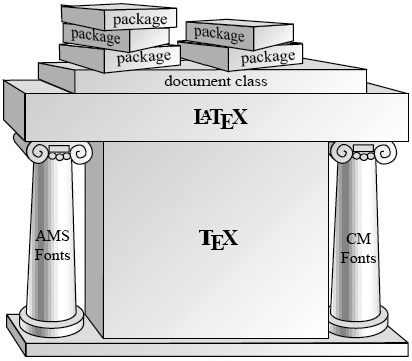
\includegraphics[width=0.45\textwidth]{latexframe}\\
      
\includegraphics[width=0.3\textwidth]{titlepage}\\%scale=0.05
      贴心\alert{秘书}
    \end{center}
  \end{columns}
\end{frame}

\begin{frame}{为什么要用\LaTeX?}{Office的那点事}%
  \centering
  
\includegraphics[height=.65\textheight]{msoffice2013.png}\\[.5em]
  \msoffice{} \footnote[frame,1]{及其类似软件(LibreOffice, etc.)}%为了在
                                %beamer中显示脚注,需要使用参数[frame]
  功能异常强大\ldots
\end{frame}

% \begin{frame}{为什么要用\LaTeX?}{与Word比较}
%   \begin{itemize}
%   \item 使用难度
%   \end{itemize}
%   \centering
%   \vspace{2ex}
%   \begin{tikzpicture}[scale=0.9, every node/.style={scale=0.9}]
%     \pgfplotsset{every axis/.append style={line width=1pt}}
%     \begin{axis}[%
%       axis x line=bottom,
%       axis y line=left,
%       ymin=0,
%       xtick={},
%       xticklabels={},
%       xlabel near ticks,
%       ytick={},
%       yticklabels={},
%       ylabel near ticks,
%       xlabel={文档大小和复杂性\footnote[frame]{\href{http://www.pinteric.com/miktex.html}{Marko
%       Pinteric: http://www.pinteric.com/miktex.html}}},
%       ylabel={耗时和难度},
%       ]
%       \begin{scope}[decoration={random steps,segment length=1pt,amplitude=0.1pt},decorate]
%         \addplot [msofficecolour, samples=130, domain=0:2] {1+2*x^3}
%                   node[near end, sloped, above] {\msoffice}
%                   node[anchor=east, pos=.98] {\tiny (我不玩了!再见\ldots)};
%          \addplot [latexcolour, samples=130, domain=0:2] {2+x}
%                   node[near end, sloped, above] {\latex};
%       \end{scope}
%     \end{axis}
%   \end{tikzpicture}
% \end{frame}

% \begin{frame}{为什么要用\LaTeX?}{与Word比较}
%   \begin{itemize}
%   \item 学习曲线
%   \end{itemize}
%   \centering
%   \vspace{2ex}
%   \begin{tikzpicture}[scale=0.9, every node/.style={scale=0.9}]
%     \pgfplotsset{every axis/.append style={line width=1pt}}
%     \begin{axis}[%
%       axis x line=bottom,
%       axis y line=left,      
%       xtick={},
%       xticklabels={},
%       xlabel near ticks,
%       ytick={},
%       yticklabels={},
%       ylabel near ticks,
%       xlabel={需求复杂度/经验},
%       ylabel={学习难度},
%       xmin=0,
%       xmax=4,
%       ymin=0,
%       ymax=4,
%       ]
%       % 用贝塞尔曲线(Bézier curve)绘制学习曲线示意图
%       \begin{scope}[decoration={random steps,segment length=1pt,amplitude=0.1pt},decorate]
%         \draw[color=msofficecolour] (0,0) .. controls (3.8,0.00) and (1.5,3.8)
%         .. (3.8,3.8) node[near end, sloped, above] {\msoffice};
%         \draw[latexcolour] (0,0) .. controls (0.1,1.8) and (1.8,1.8)
%         .. (3.8,1.6) node[xshift = -0.8cm, sloped, above] {\latex};
%       \end{scope}
%     \end{axis}
%   \end{tikzpicture}
% \end{frame}

% \begin{frame}{为什么要用\LaTeX?}{Word的那点事}
%   \stretchon
%   \begin{itemize}
%   \item \msoffice 是 \wysiwyg
%     \begin{itemize}
%     \item ``\textsc{What You See Is What You \emph{Get}}''
%     \item 格式和结构有时是含蓄的
%     \item 貌似易用,但对排版只能进行有限的控制
%     \end{itemize}
%     %\myrule
%   \item \latex 是 \wysiwym
%     \begin{itemize}
%     \item ``\textsc{What You See Is What You \emph{Mean}}''
%     \item 格式与结构清晰
%     \item 貌似繁琐,实则是对版面可以进行详细的控制
%     \end{itemize}
%   \end{itemize}
%   \stretchoff
% \end{frame}

% \begin{frame}{为什么要用\LaTeX?}{Word的那点事}
%   \stretchon
%   \begin{itemize}
%   \item 玻璃瓶和塑料瓶
%     \begin{itemize}
%     \item \msoffice 是玻璃瓶$\Rightarrow$ \alert{易碎}
%     \item \latex 是塑料瓶$\Rightarrow$ \alert{皮实}
%     \end{itemize}
%   \item 模板
%     \begin{itemize}
%     \item \msoffice 往往是\alert{规定}$\Rightarrow$ 沦落为低级趣味的\alert{格式刷}
%     \item \latex 强制使用模板$\Rightarrow$ 真正实现了\alert{内容与格式的分离}
%     \end{itemize}
%   \item 轮子的故事
%     \begin{itemize}
%     \item \msoffice$\Rightarrow$ \alert{ 发明和制造}轮子
%     \item \latex$\Rightarrow$  \alert{ 使用}轮子
%     \end{itemize}
%   \item 两条腿走路
%     \begin{itemize}      
%     \item 不会用
%       \begin{itemize}
%       \item \msoffice $\Rightarrow$ 文档难看,格式丑
%       \item \latex $\Rightarrow$ 无法编译,\alert{没有文档}
%       \end{itemize}
%     \item 会用
%       \begin{itemize}
%       \item \msoffice $\Rightarrow$ \alert{难看}的文档
%       \item \latex $\Rightarrow$ 漂亮的文档
%       \end{itemize}
%     \item 用的好
%       \begin{itemize}
%       \item \msoffice $\Rightarrow$ \alert{完美}的文档
%       \item \latex $\Rightarrow$ \alert{完美}的文档
%       \end{itemize}
%     \end{itemize}    
%   \end{itemize}
%   \stretchoff
% \end{frame}

%%% Local Variables:
%%% mode: latex
%%% TeX-master: "../main.tex"
%%% End:
